% Main Text (Page One)
Prime numbers are integers greater than 1 that have no positive divisors other than 1 and themselves. They form the multiplicative building blocks of arithmetic. The first few primes — 2, 3, 5, 7, 11, 13, 17, 19, 23, 29 — occur without any obvious pattern. Their spacing varies. While exact expressions for the $n$th prime can be written, they do not yield new primes without some form of explicit primality testing.\footnote{It is difficult to make an accurate statement about whether there exists a "formula" for the primes. Terms like "closed-form" lack a consistent definition. There are prime-generating polynomials (with caveats), formal summation formulas, and tautological definitions such as $p_n = \min\{k \in \mathbb{N} : k > p_{n-1} \text{ and } k \text{ is prime}\}$. See, for example, the entries on prime formulas at MathWorld.}


As numbers increase, primes become less frequent. The Prime Number Theorem formalizes this observation: the number of primes less than $x$ grows approximately like $x / \log x$. This gives an average spacing between primes near $x$ of about $\log x$, but does not constrain individual gaps.

The differences between consecutive primes can be small or large. Pairs such as (3, 5), (5, 7), (11, 13), (17, 19), and (29, 31) each differ by 2. The smallest prime gap of 2 recurs often at the start of the number line. By contrast, the primes 370,261 and 370,373 are separated by 112, with no primes between them. In general, for any given $N$, there exist consecutive primes with gap larger than $N$. One construction uses the sequence $
(n+1)! + 2,  (n+1)! + 3,  \dots,  (n+1)! + (n+1)$, which yields $n$ consecutive composite numbers, hence a gap of at least $n$ between the bounding primes.

What remains unknown is whether specific small gaps — such as a fixed difference of 2 — occur infinitely often. The Twin Prime Conjecture asserts that there are infinitely many primes $p$ such that $p + 2$ is also prime. This remains one of the major unproved conjectures in number theory.

In 2013, Yitang Zhang proved that there exists a constant $B$ such that infinitely many pairs of distinct primes differ by at most $B$. His original bound was $B < 70{,}000{,}000$. While this does not resolve the twin prime conjecture, it proves that small prime gaps occur infinitely often and that prime gaps do not grow without limit.

Zhang's method extended earlier work by Goldston, Pintz, and Yıldırım. He combined improved estimates on the distribution of primes in arithmetic progressions with a weighted sieve construction that amplified configurations where multiple primes appear close together. This yielded an explicit, finite bound on the gap size that recurs infinitely often.

Following Zhang's proof, the Polymath8 collaboration reduced the bound from 70 million to below 250 through analytic refinements. Later on, James Maynard introduced a simplified sieve method that removed the need for strong distributional estimates and extended the technique to detect multiple primes within bounded intervals.

Zhang's result drew attention not only for its mathematical content, but also for the circumstances of its discovery. After completing his doctorate, he spent many years outside academic mathematics, with no permanent university position and limited research output. His proof was written and submitted independently, without collaborators or institutional support. The publication of his result led to rapid follow-up work, large-scale collaboration, and the re-entry of a long-standing problem into the mathematical mainstream.

Although the Twin Prime Conjecture remains unresolved, the question of whether bounded prime gaps recur has been answered. There exists a finite value — currently known to be less than 250 — that bounds infinitely many consecutive prime gaps.

Prime gaps do not merely recur within fixed bounds. They can also grow arbitrarily large. This follows from the construction of long sequences of consecutive composite numbers. For example, the integers $(n+1)! + 2,  (n+1)! + 3,  \dots,  (n+1)! + (n+1)$ are all divisible by $2$ through $(n+1)$ respectively and therefore contain no primes. Since the factorial term dominates, these $n$ consecutive composites yield a prime gap of length at least $n$. This provides a lower bound that increases with $n$, and hence with $x$.

Prime gaps are not constrained from above. For any natural number $N$, there exist consecutive prime numbers that are separated by a gap greater than $N$. This fact can be shown through explicit construction. Consider the numbers $(n+1)! + 2,  (n+1)! + 3,  \dots,  (n+1)! + (n+1).$ Each of these is divisible by one of the integers $2, 3, \dots, n+1$ and is therefore composite. The primes immediately before and after this block are separated by at least $n$ steps. As $n$ increases, the size of the gap increases. This shows that prime gaps can be made arbitrarily large.

More generally, mathematicians study how large these gaps can become as the numbers involved grow. Let $G(x)$ be the largest gap between consecutive primes less than $x$. It is known that $G(x)$ increases faster than $\log x$, which is the average spacing predicted by the Prime Number Theorem. A classical result due to Paul Erdős shows that $G(x)$ exceeds a constant multiple of $\log x$ times another slowly growing function. This means that although most prime gaps are relatively small, unusually large gaps must still occur infinitely often. The best known upper bounds on $G(x)$ remain far from matching the lower bounds. Some of the strongest predictions, such as Cramér's conjecture, suggest that the maximal gap should grow no faster than $\log^2 x$, but this has not been proved.

Alongside these increasingly long gaps, primes also form highly regular patterns. In 2004, Ben Green and Terence Tao proved that the primes contain arbitrarily long arithmetic progressions. For any integer $k$, there exists a sequence of the form $p,  p + d,  p + 2d,  \dots,  p + (k - 1)d$ in which all terms are prime. The length $k$ can be taken as large as desired. Although such progressions become rarer as $k$ increases, the result shows that they never stop appearing.

The Green–Tao theorem adapts tools from ergodic theory and additive combinatorics. It begins by approximating the set of primes using related sequences whose behavior is easier to control. A transference principle then carries structural results from these surrogate sequences back to the primes themselves. The original result was later extended by Green and Ziegler to cover polynomial progressions, such as $p,  p + q,  p + 4q,  p + 9q,  p + 16q, $ in which the differences between terms follow a fixed polynomial pattern and all terms are again required to be prime.

These discoveries do not contradict the decreasing density of the primes. The proportion of primes among all integers goes to zero as numbers grow. But even within this sparsity, the primes retain internal arithmetic structure. Long gaps and long progressions both occur. Some primes are isolated; others appear in alignment. The apparent randomness of their distribution does not eliminate deep regularities.

Many questions about the distribution of primes, including the spacing between them and the occurrence of structured patterns, remain unresolved. Some of these questions cannot be settled with current methods because their answers depend on an open conjecture in complex analysis and number theory. This conjecture is known as the Riemann Hypothesis.

The Riemann Hypothesis (RH) concerns a function called the Riemann zeta function. This function is initially defined as a sum over positive integers, $\zeta(s) = \sum_{n=1}^\infty \frac{1}{n^s},$
which converges when the complex number $s$ has real part greater than $1$. Through a process known as analytic continuation, the function can be extended to other values of $s$ in the complex plane. The hypothesis asserts that all nontrivial zeros of $\zeta(s)$ — that is, all values of $s$ for which $\zeta(s) = 0$ and which are not negative even integers — lie on the vertical line $\mathrm{Re}(s) = \tfrac{1}{2}$.

Assuming RH, many bounds on the error terms in prime-counting functions become significantly tighter. For example, the difference between the actual number of primes up to $x$ and the estimate $x / \log x$ can be bounded more sharply. The hypothesis also leads to improved estimates on how often primes occur in short intervals and how large the gaps between consecutive primes can be. Without a proof, many of these refinements remain conditional. The Riemann Hypothesis has been verified for many individual zeros through numerical computation, and no counterexamples have been found. Nevertheless, the general statement remains unproved.


\begin{commentary}[Commentary: Transparent Statements, Resistant Proofs]
The central claim of this chapter can be stated in one line and requires no definitions beyond the integers. This is typical of many problems in number theory. Simplicity of formulation does not imply tractability.

Zhang's proof is concise but not elementary. Its validity depends on a precise balance between distributional estimates and sieve structure. Subsequent refinements by the Polymath8 project, led by Terence Tao, and by Maynard's independent method reduced the bound but did not simplify the analytic core.

This chapter is included because of Zhang's personal trajectory and because it illustrates a broader principle: many problems in number theory are easy to state and test numerically, yet remain inaccessible to current methods.
\end{commentary}

\clearpage
\vspace*{\stretch{1}}

\begin{center}
  {\Large \textbf{Twelve Open Problems in Additive Prime Number Theory}}

  \vspace{0.5em}
  \textit{These twelve problems concern the additive structure and distribution of primes. All remain unresolved.}

  \vspace{1em}

  \begin{tcolorbox}[
    colback=gray!2,
    colframe=gray!60,
    boxrule=0.4pt,
    width=\textwidth,
    arc=1pt,
    left=6pt,
    right=6pt,
    top=6pt,
    bottom=6pt,
    shadow={0mm}{-0.5mm}{0mm}{gray!40}
  ]
  \setstretch{1}

  \noindent\begin{minipage}{0.44\textwidth}
    \textbf{1. Twin Prime Conjecture}\\
    \emph{Are there infinitely many primes \(p\) such that \(p+2\) is also prime?}\\
    \hfill\textsc{Alphonse de Polignac, 1846}
  \end{minipage}\hfill
  \begin{minipage}{0.44\textwidth}
    \textbf{2. Goldbach's Conjecture}\\
    \emph{Is every even number greater than 2 the sum of two primes?}\\
    \hfill\textsc{Christian Goldbach, 1742}
  \end{minipage}

  \vspace{2em}

  \noindent\begin{minipage}{0.44\textwidth}
    \textbf{3. de Polignac's Conjecture}\\
    \emph{Does every even number \(2k\) occur infinitely often as a prime gap?}\\
    \hfill\textsc{Alphonse de Polignac, 1846}
  \end{minipage}\hfill
  \begin{minipage}{0.44\textwidth}
    \textbf{4. Oppermann's Conjecture}\\
    \emph{Is there always a prime between \(n(n - 1)\) and \(n^2\), and another between \(n^2\) and \(n(n + 1)\)?}\\
    \hfill\textsc{Ludwig Oppermann, 1882}
  \end{minipage}

  \vspace{2em}

  \noindent\begin{minipage}{0.44\textwidth}
    \textbf{5. Erdős–Turán on Additive Bases}\\
    \emph{Does every set \(A\) with divergent \(\sum 1/a\) satisfy \(A + A\) contains all large integers?}\\
    \hfill\textsc{Erdős and Turán, 1941}
  \end{minipage}\hfill
  \begin{minipage}{0.44\textwidth}
    \textbf{6. Prime Summation Thresholds}\\
    \emph{What is the minimal \(s\) such that every large even number is a sum of \(s\) primes?}\\
    \hfill\textsc{I.M. Vinogradov, 1937}
  \end{minipage}

  \vspace{2em}

  \noindent\begin{minipage}{0.44\textwidth}
    \textbf{7. Cramér's Conjecture}\\
    \emph{Is the maximal prime gap \(O((\log p)^2)\)?}\\
    \hfill\textsc{Harald Cramér, 1936}
  \end{minipage}\hfill
  \begin{minipage}{0.44\textwidth}
    \textbf{8. Firoozbakht's Conjecture}\\
    \emph{Is the sequence \(p_n^{1/n}\) strictly decreasing?}\\
    \hfill\textsc{Farideh Firoozbakht, 1982}
  \end{minipage}

  \vspace{2em}

  \noindent\begin{minipage}{0.44\textwidth}
    \textbf{9. Legendre's Conjecture}\\
    \emph{Is there always a prime between \(n^2\) and \((n+1)^2\)?}\\
    \hfill\textsc{A.-M. Legendre, 1798}
  \end{minipage}\hfill
  \begin{minipage}{0.44\textwidth}
    \textbf{10. Lemoine's Conjecture}\\
    \emph{Is every odd number greater than 5 the sum of a prime and twice another prime?}\\
    \hfill\textsc{Émile Lemoine, 1895}
  \end{minipage}

  \vspace{2em}

  \noindent\begin{minipage}{0.44\textwidth}
    \textbf{11. Andrica's Conjecture}\\
    \emph{Does \(\sqrt{p_{n+1}} - \sqrt{p_n} < 1\) hold for all \(n\)?}\\
    \hfill\textsc{Dorin Andrica, 1986}
  \end{minipage}\hfill
  \begin{minipage}{0.44\textwidth}
    \textbf{12. Erdős–Straus Conjecture}\\
    \emph{Is \(\tfrac{4}{n} = \tfrac{1}{a} + \tfrac{1}{b} + \tfrac{1}{c}\) solvable in integers for all \(n\ge2\)?}\\
    \hfill\textsc{Erdős and Straus, 1948}
  \end{minipage}

  \end{tcolorbox}
\end{center}

\vspace*{\stretch{1}}

\thispagestyle{empty}
\begin{figure}[p]
\centering
\fbox{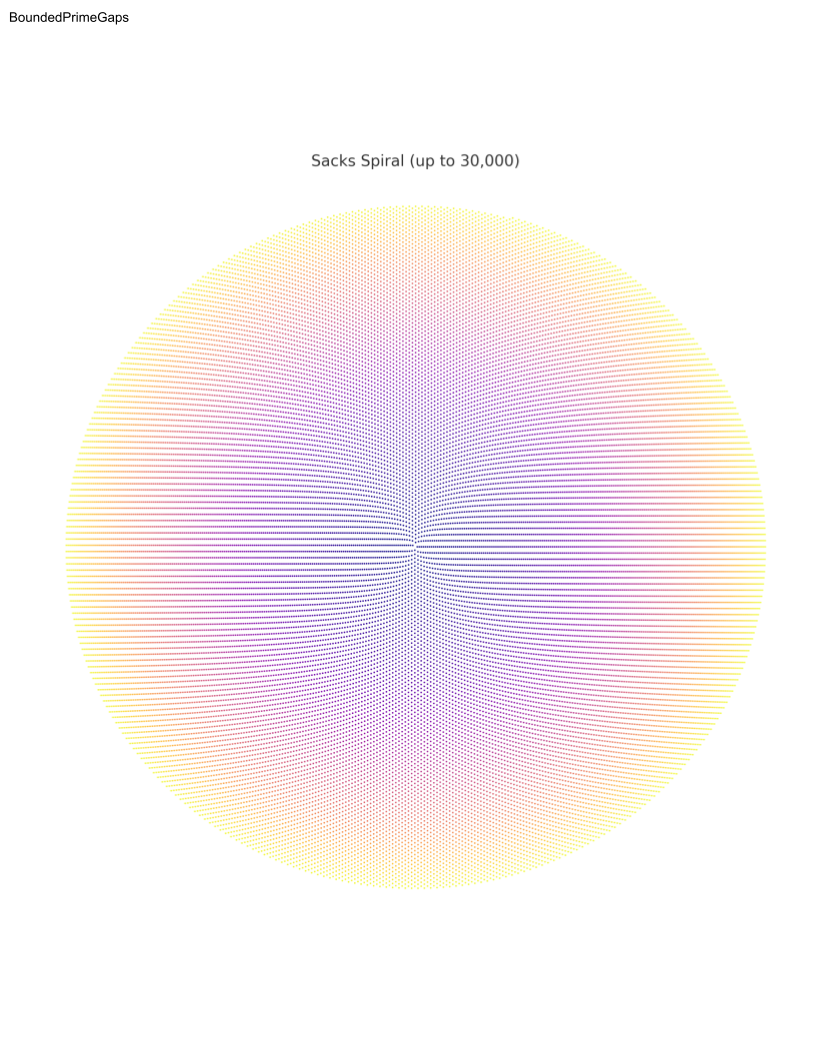
\includegraphics[width=\textwidth,height=\textheight,keepaspectratio]{08_BoundedPrimeGaps/sacks_illu.png}}
\end{figure}

\begin{SideNotePage}{

  \textbf{Top panel:} Natural numbers 1-25 with primes (red) and composites (teal), showing twin prime pairs like (3,5), (5,7), (11,13), (17,19).
  \newline
  \textbf{Second panel:} Consecutive primes with gap sizes marked by blue arrows, from the minimal gap of 2 to larger separations like 8 between 23 and 31.
  \newline
  \textbf{Third panel:} Scatter plot of prime gaps $p_{n+1} - p_n$ versus $p_n$ for the first 10,000 primes, showing most gaps are small with rare large exceptions. Reference lines mark key bounds: twin primes (gap = 2), Polymath8's refined bound (246), and Zhang's original breakthrough (70 million). Infinitely many gaps stay below some fixed bound, guaranteeing points always appear below these lines.
  
  Note the key distinction: for small gaps we seek absolute bounds (fixed numbers like 246), while for large gaps the bounds are functions of $p_n$ that grow as primes get larger.
  
  \textbf{Bottom panel:} How large can prime gaps become? This shows the largest observed gaps (light blue) compared to theoretical predictions. The red lines show upper bound conjectures for maximum gap size, while colored lower bounds prove that gaps must occasionally be large. The scatter demonstrates that while most gaps are small relative to the local prime density, some gaps are much larger than the typical spacing in their region.
}{08_BoundedPrimeGaps/prime_gaps_combined.pdf}
\end{SideNotePage}